% PIC: @Oktavian19
\begin{titlepage}
  \thispagestyle{empty}
  \begin{tikzpicture}[remember picture, overlay]
    \node[inner sep=0pt] at (current page.center) {%
      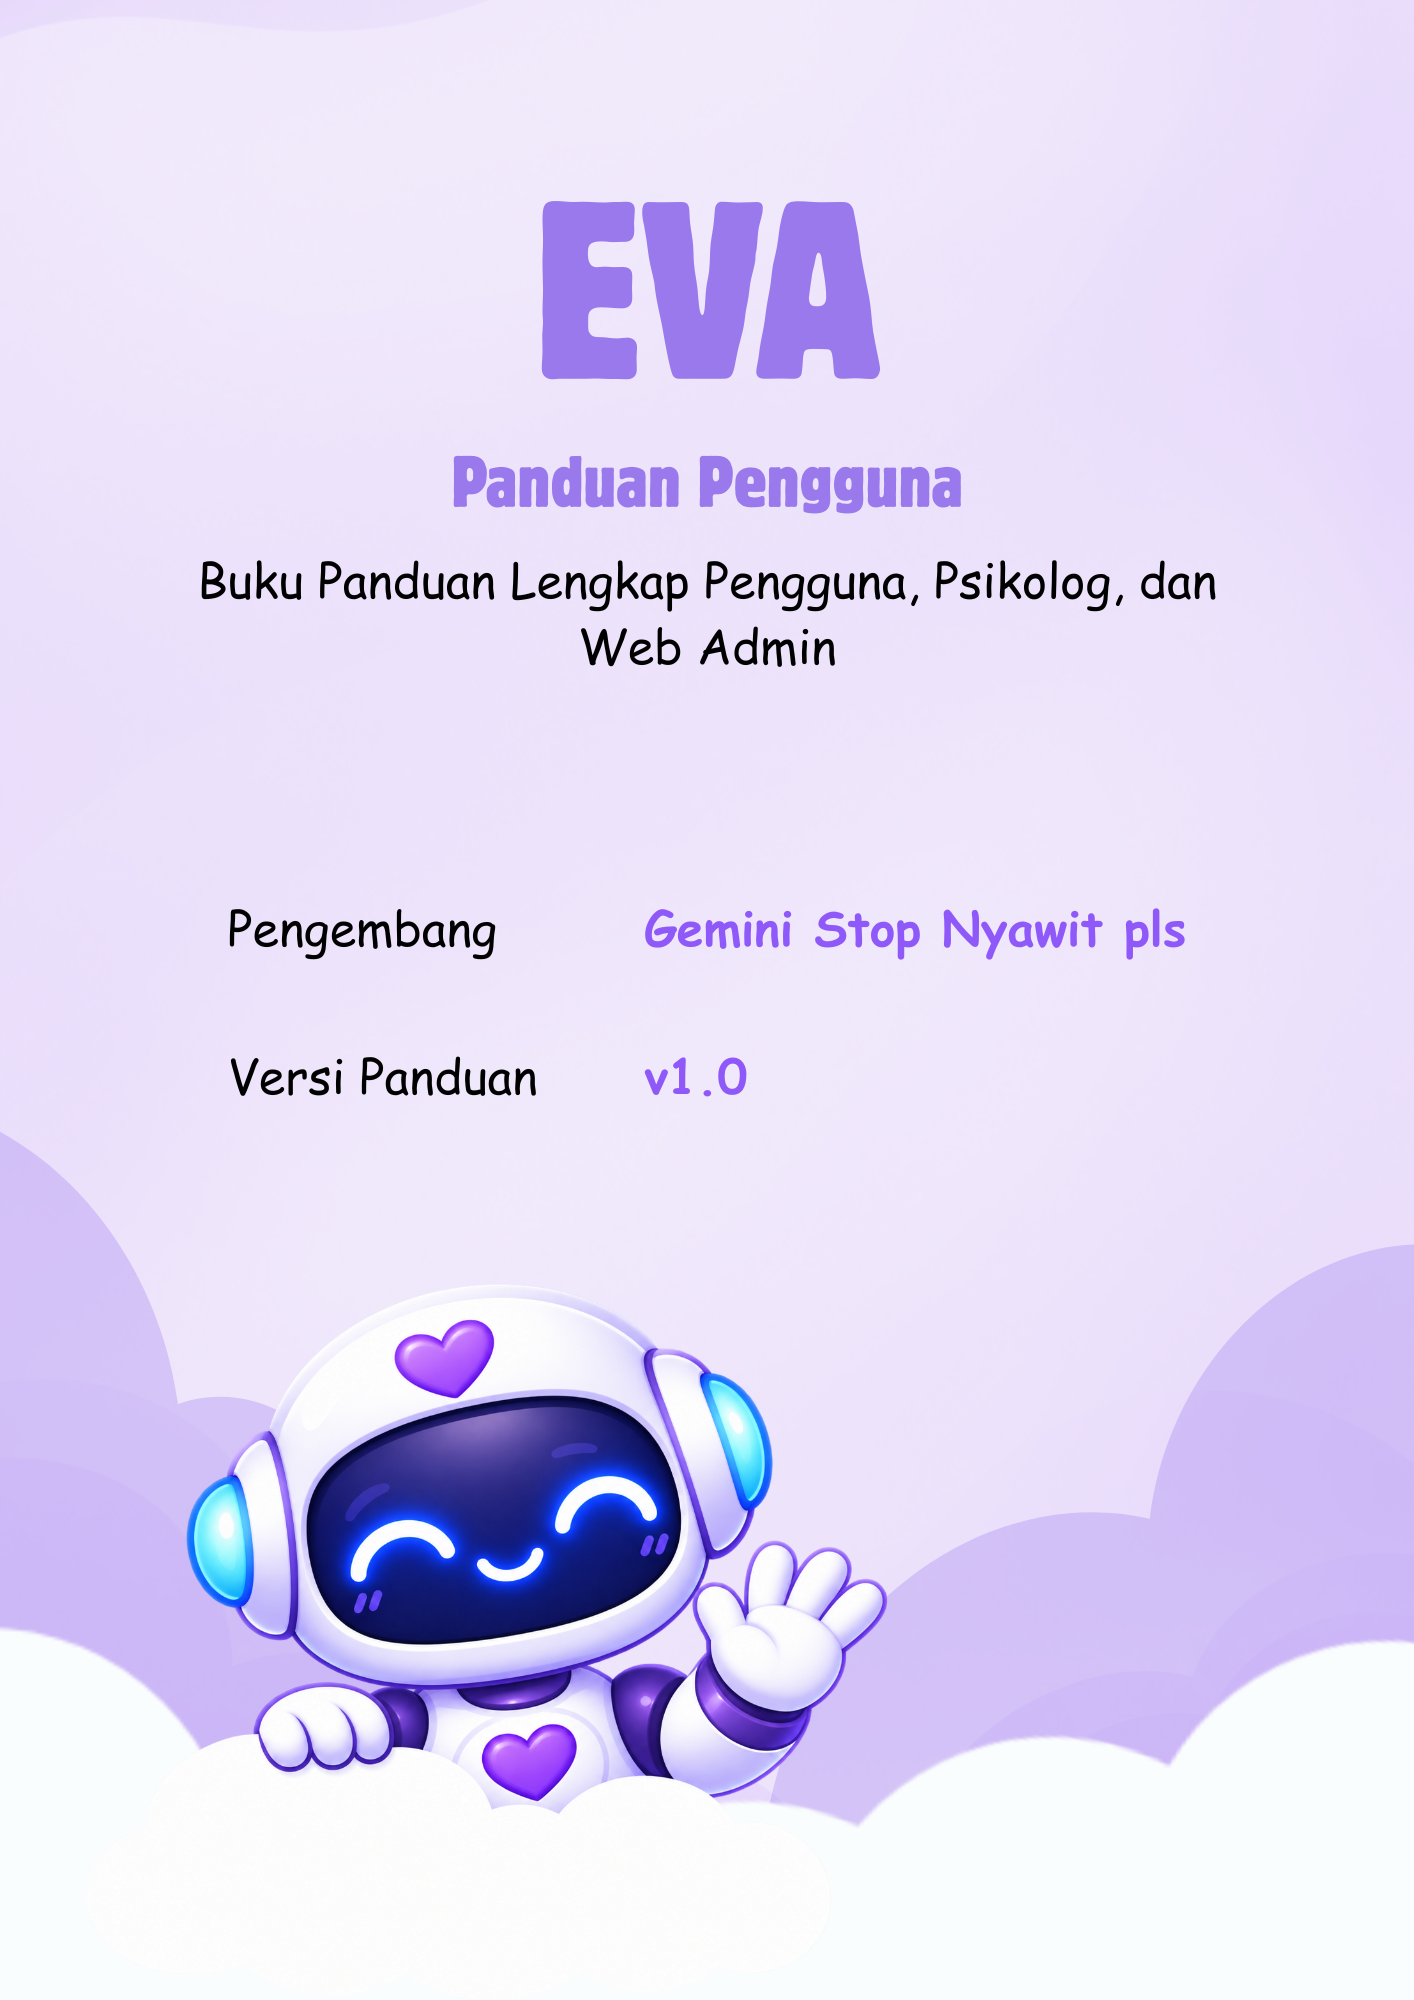
\includegraphics[width=\paperwidth,height=\paperheight]{figures/shared/cover_panduan.png}%
    };
  \end{tikzpicture}
  \mbox{}
  \clearpage
\end{titlepage}

\chapter*{Kata Pengantar dan Konvensi Panduan}
\addcontentsline{toc}{chapter}{Kata Pengantar dan Konvensi Panduan}

Buku panduan ini disusun sebagai rujukan operasional resmi untuk seluruh aktor di dalam \textbf{EVA Ecosystem}, mencakup aplikasi \textbf{EVA Mobile} (untuk pengguna atau pasien), \textbf{EVA Counselor} (untuk psikolog dan konselor berlisensi), serta \textbf{Web Portal dan Admin} (untuk informasi publik dan pengelolaan operasional platform).

\section*{Cara Menggunakan Buku Ini}
\begin{itemize}[leftmargin=1.4em]
  \item \textbf{Pengguna Umum / Pasien}: Fokus pada Bab~\ref{chap:pendahuluan}, Bab~\ref{chap:memulai-akun}, Bab~\ref{chap:eva-mobile}, serta Bab~\ref{chap:privasi-etika}.
  \item \textbf{Psikolog / Konselor Mitra}: Fokus pada Bab~\ref{chap:pendahuluan}, Bab~\ref{chap:memulai-akun}, Bab~\ref{chap:eva-counselor}, Bab~\ref{chap:alur-lintas-aktor}, dan Bab~\ref{chap:privasi-etika}.
  \item \textbf{Administrator Platform}: Fokus pada Bab~\ref{chap:web-portal-admin}, Bab~\ref{chap:alur-lintas-aktor}, dan Bab~\ref{chap:troubleshooting-faq}.
\end{itemize}

\section*{Konvensi Penulisan}
\calloutnote{Catatan Informasi}{Kotak berwarna indigo berisi penjelasan konteks sistem, aturan bisnis, atau definisi alur kerja yang perlu dipahami sebelum menjalankan aksi.}
\callouttip{Tips Operasional}{Kotak berwarna hijau berisi saran praktik terbaik untuk mempercepat pekerjaan dan mencegah kesalahan input.}
\calloutwarn{Peringatan Penting}{Kotak berwarna kuning/oranye menandai aksi sensitif yang memengaruhi keamanan akun, kepatuhan etika klinis, atau transaksi keuangan.}
